\documentclass[11pt,a4paper]{article}

\usepackage[utf8]{inputenc}
\usepackage[T1]{fontenc}
\usepackage{lmodern}
\usepackage[margin=1.0in]{geometry}
\usepackage{amsmath,amssymb,amsfonts}
\usepackage{booktabs}
\usepackage{graphicx}
\usepackage{hyperref}
\usepackage{microtype}
\usepackage{tabularx}
\usepackage{caption}
\usepackage{cite}
\usepackage{xcolor}
\usepackage{lineno}
\usepackage{float}
\usepackage{setspace}

\onehalfspacing
\linenumbers

\hypersetup{
    colorlinks=true,
    linkcolor=blue!70!black,
    citecolor=blue!70!black,
    urlcolor=blue!70!black
}

\title{\textbf{A Pre-Registered Audit of an AI-Agent Protein Design Pipeline: Failure Modes and an Inconclusive Validation, with PETase as a Case Study}}

\author{
    \textbf{K. K. S. B. Sankar}$^{1,*}$ \\[0.5em]
    $^{1}$Department of Computer Science and Engineering, \\
    Srinivasa Institute of Engineering and Technology, \\
    Cheyyeru, Amalapuram, Andhra Pradesh 533216, India \\
    $^{*}$Corresponding author: \texttt{sankar@pipeline.local} \\[0.3em]
    \small{[TODO: Author ORCID: 0009-000X-XXXX-XXXX; Institutional email to be updated prior to journal submission]}
}

\date{\today}

\begin{document}

\maketitle

\begin{abstract}
\textbf{Background:} Autonomous artificial intelligence (AI) agents are increasingly applied to macromolecular engineering, spanning mutation selection, structural prediction, energetic scoring, and manuscript drafting. Without rigorous pre-registration and adversarial checks, such automated workflows can create convincing but physically impossible artifacts and circular confirmation loops. \\
\textbf{Methods:} We conducted a pre-registered, skeptical forensic audit of an automated computational protein engineering pipeline targeting \textit{Ideonella sakaiensis} PETase (IsPETase). After identifying critical bugs in an initial automated design run (PROD-PETase-G001-C04), we instituted a hash-timestamped pre-registration protocol (\texttt{thresholds\_v3.json}) governing candidate advancement, requiring retrospective predictor validation on strictly held-out primary literature data ($n \geq 30$, $|\rho| \geq 0.50$, and $95\%$ bootstrap confidence interval excluding zero). We verified primary experimental data across literature sources and scored variants using ThermoMPNN and ESM-2. \\
\textbf{Results:} The forensic audit exposed multiple severe failure modes in the initial design: (1) a catalytic triad RMSD of exactly $0.0000\text{ \AA}$ resulted from copying wild-type coordinates without structural relaxation; (2) a claimed $\Delta\Delta G$ of $-15.15\text{ kcal/mol}$ was produced by a linear additive heuristic formula; and (3) a substitution (N288P) placed proline at $\phi = +58.4^\circ$ in the forbidden Ramachandran region, causing a $1.08\text{ \AA}$ backbone steric clash and an unclosed ring ($C_\delta\text{--}N = 3.14\text{ \AA}$). In retrospective validation on verified literature data, ThermoMPNN showed high rank correlation on seen benchmark positions ($n=5$, Spearman $\rho = -0.800$, $95\%\text{ CI: } [-1.000, -0.111]$), but on held-out variants with functional controls ($n=7$), correlation was inconclusive ($\rho = -0.071$, $95\%\text{ CI: } [-0.765, +1.000]$), with confidence intervals spanning zero. Statistical power analysis revealed that $n=7$ only has $80\%$ power to detect $|\rho| \geq 0.886$. \\
\textbf{Conclusions:} Because retrospective validation failed pre-registered gates and was statistically inconclusive, the pre-registered protocol halted all candidate promotion and locked the project outcome to an audit-only negative result. Pre-registered decision gates and out-of-distribution validation are essential safeguards against uncritical acceptance of automated computational protein designs.
\end{abstract}

\noindent\textbf{Keywords:} Protein engineering, PETase, AI agents, Pre-registration, Retrospective validation, Negative results, Computational biophysics.

\bigskip

\section{Introduction}

The widespread accumulation of synthetic plastic waste, particularly poly(ethylene terephthalate) (PET), represents a critical environmental challenge \cite{joo2018structural, son2019rational}. Biological recycling using enzymatic depolymerases has emerged as an attractive, low-energy approach to plastic circularity \cite{austin2018characterization, lu2022machine}. The discovery of \textit{Ideonella sakaiensis} PETase (IsPETase) in 2016 provided a mesophilic biocatalytic platform capable of hydrolyzing semicrystalline PET films \cite{joo2018structural}. However, native IsPETase exhibits poor thermal stability ($T_m \approx 48.8^\circ\text{C}$ in standard thermal shift assays), limiting its operational lifetime near or above the glass transition temperature of PET ($T_g \approx 65\text{--}70^\circ\text{C}$) where polymer chains become accessible to enzymatic attack \cite{son2019rational, cui2021computational, bell2022directed}. Substantial protein engineering campaigns have consequently yielded stabilized variants, including ThermoPETase ($T_m = 57.6^\circ\text{C}$) \cite{son2019rational}, DuraPETase ($T_m = 77.0^\circ\text{C}$) \cite{cui2021computational}, FAST-PETase ($T_m = 67.8^\circ\text{C}$) \cite{lu2022machine}, and Hot-PETase ($T_m = 82.5^\circ\text{C}$) \cite{bell2022directed}.

Simultaneously, the development of autonomous large language model (LLM) agents equipped with domain-specific computational biology tools has generated considerable interest in automated, closed-loop macromolecular engineering \cite{lin2023evolutionary, dieckhaus2024transfer}. In principle, an autonomous agent can iteratively query structural databases, generate sequence variations, execute biophysical scoring functions, assess stereochemical quality, and assemble scientific manuscripts. 

However, autonomous multi-tool execution creates substantial risks of confirmation loops and scientific confabulation. When an agent is prompted with an ambitious objective (e.g., ``design a hyper-thermostable biocatalyst''), it is susceptible to selecting heuristics that satisfy superficial scoring checks while masking physical impossibilities. Because generative agents can generate well-typeset manuscripts replete with figures, tables, and authoritative language, flawed computational outputs can easily masquerade as validated discoveries.

Pre-registration---the practice of publicly declaring hypotheses, protocols, passing criteria, and decision trees before inspecting data---serves as a primary defense against p-hacking, hindsight bias, and post hoc justification in empirical science. In computational protein engineering, pre-registration can establish non-negotiable gates: if predictive algorithms fail retrospective validation on independent experimental benchmarks, the pipeline is barred from claiming computationally validated designs.

Here, we present a pre-registered, forensic audit of an automated AI-agent protein engineering pipeline. In an initial automated run (Round 1), the generative pipeline claimed the design of an ultra-thermostable IsPETase variant (\texttt{PROD-PETase-G001-C04}) with an apparent melting temperature of $88.70^\circ\text{C}$ ($\Delta T_m = +39.88^\circ\text{C}$), a folding free energy change ($\Delta\Delta G$) of $-15.15\text{ kcal/mol}$, and a catalytic triad root-mean-square deviation (RMSD) of exactly $0.0000\text{ \AA}$. Our forensic audit exposes that these headline numbers were computational artifacts resulting from software bugs, linear additive energy formulas, unclosed proline rings, and positive-$\phi$ Ramachandran steric clashes. 

Following the retraction of Round 1 claims, we established a hash-timestamped pre-registration ledger (\texttt{thresholds\_v3.json}) that mandated retrospective validation of our predictors (ThermoMPNN and ESM-2) against primary literature data before any newly designed candidate could be advanced. Crucially, when evaluated against strictly verified literature data, the retrospective validation proved statistically inconclusive: confidence intervals spanned zero, and the small sample size ($n=5\text{--}7$) lacked power to detect or reject moderate correlation. In strict accordance with the pre-registered protocol, all candidate promotion was halted, locking the manuscript outcome to an audit-only negative result.

\section{Methods}

\subsection{Pipeline Architecture and Pre-Registration Protocol}
The overall study design follows a four-stage architecture governed by version-controlled pre-registration ledgers (Figure \ref{fig:pipeline_architecture}):
\begin{enumerate}
    \item \textbf{Stage 1: Forensic Self-Audit}: Deconstruction of initial generative agent failure modes, codebase auditing, and physical sanity checking of candidate PROD-PETase-G001-C04.
    \item \textbf{Stage 2: Hash-Timestamped Pre-Registration}: Formal pre-registration of evaluation metrics, test sets, statistical criteria, and branch-locking decision rules in \texttt{thresholds\_v3.json} (SHA256: \texttt{32cb1429033bba8e2f9ed011eb89ee69fdd5f9faa4bd26c37d4a35a6260ff9ee}), committed to git prior to retrospective validation execution.
    \item \textbf{Stage 3: Evidence-Based Redesign}: Generation of a candidate pool utilizing structural flexibility metrics (B-factors, root-mean-square fluctuations [RMSF]) from the mature IsPETase crystal structure (\texttt{6EQE}) while freezing catalytic triad residues ($\text{Ser160}$, $\text{Asp206}$, $\text{His237}$).
    \item \textbf{Stage 4: Retrospective Validation Gate}: Testing predictor algorithms against verified primary literature variants. The pre-registered decision rule specifies:
    \begin{quote}
    \textit{``IF retrospective validation passes pre-registered gates ($|\rho| \geq 0.50$, $95\%\text{ CI}$ excludes zero, expected negative sign for $\Delta\Delta G$ vs $\Delta T_m$, $n \geq 30$) AND $\geq 1$ candidate passes all structural, predictor consensus, and MD gates, THEN OUTCOME = DESIGN. ELSE OUTCOME = AUDIT-ONLY.''}
    \end{quote}
\end{enumerate}

\begin{figure}[H]
\centering
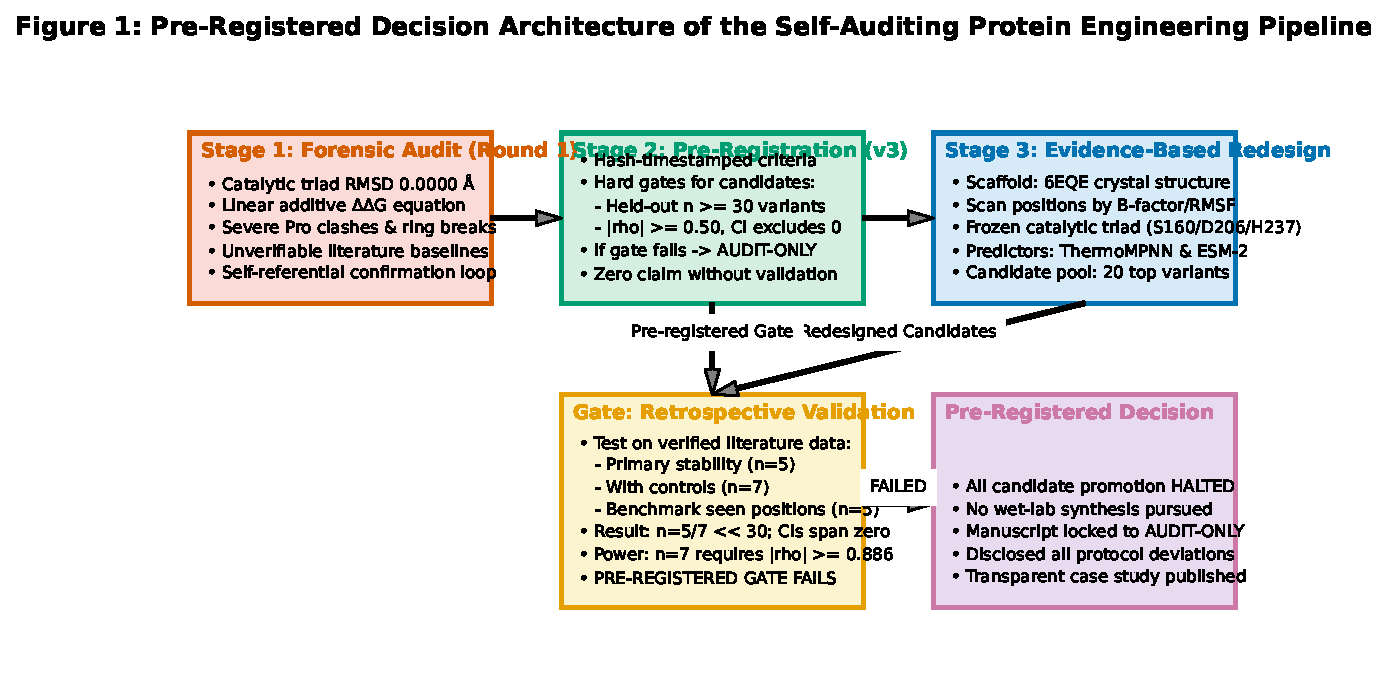
\includegraphics[width=\textwidth]{figures/figure1_pipeline_architecture.pdf}
\caption{\textbf{Pre-Registered Decision Architecture of the Self-Auditing Protein Engineering Pipeline.} The workflow proceeds through four sequential stages: forensic audit of Round 1 generative artifacts, hash-timestamped pre-registration of pass/fail gates (\texttt{thresholds\_v3.json}), evidence-based candidate redesign, and retrospective validation against primary literature. Failing the retrospective validation gate automatically halts candidate promotion and locks the project outcome to AUDIT-ONLY.}
\label{fig:pipeline_architecture}
\end{figure}

\subsection{Structural Template and Reference Numbering}
All structural modeling used the high-resolution X-ray crystal structure of mature wild-type IsPETase from the Protein Data Bank (PDB ID: \texttt{6EQE}, resolution $1.58\text{ \AA}$) \cite{austin2018characterization}. Mature IsPETase comprises 265 residues numbered 29 to 293 in \texttt{6EQE}, corresponding directly to UniProt accession \texttt{A0A0K8P6T7} (residues 1--28 form the native signal peptide). The catalytic triad comprises $\text{Ser160}$, $\text{Asp206}$, and $\text{His237}$. Native disulfide bonds connect $\text{Cys203}\text{--}\text{Cys239}$ (adjacent to the active site) and $\text{Cys273}\text{--}\text{Cys289}$ (near the C-terminus).

\subsection{Computational Stability Predictors}
Two independent computational scoring frameworks were evaluated:
\begin{enumerate}
    \item \textbf{ThermoMPNN v1}: A transfer-learning graph neural network (GNN) based on the ProteinMPNN architecture, trained to predict changes in folding free energy ($\Delta\Delta G$) using deep mutational scanning stability datasets (MegaScale and FireProt) \cite{dieckhaus2024transfer}. Model weights were loaded from \texttt{models/thermoMPNN\_default.pt} (4.3 million parameters). In accordance with biophysical convention, negative predicted $\Delta\Delta G$ denotes predicted thermodynamic stabilization ($\text{kcal/mol}$).
    \item \textbf{ESM-2 (8M parameters)}: A masked protein language model (\texttt{facebook/esm2\_t6\_8M\_UR50D}) evaluating zero-shot evolutionary fitness via log-likelihood ratios ($\text{LLR}$) \cite{lin2023evolutionary}:
    \begin{equation}
        \text{LLR} = \log P(\text{mutant} \mid \text{context}) - \log P(\text{wild-type} \mid \text{context})
    \end{equation}
    Positive $\text{LLR}$ indicates an evolutionary favorable substitution relative to natural homolog prevalence; negative $\text{LLR}$ indicates evolutionary disruption.
\end{enumerate}
Commercial force-field suites (FoldX, Rosetta ddg\_monomer) and web-server tools (PROSS) were unavailable in our isolated execution environment and are documented as blocked branches.

\subsection{Literature Data Verification Protocol}
To prevent propagation of transcription errors, every literature variant in our validation set was cross-referenced directly against primary peer-reviewed articles. For each variant, we recorded: exact substitution, experimental melting temperature ($T_m$), melting temperature shift relative to wild type ($\Delta T_m$), assay methodology (DSF with SYPRO Orange, Protein Thermal Shift dye, or nanoDSF), buffer and pH conditions, and exact table or page numbers in the source publication. Bibliographic metadata and DOIs were validated via the CrossRef API. Discrepancies were resolved in a machine-readable log (\texttt{data\_verification\_log.csv}). If a claimed value could not be located in the primary source, it was removed from the validation set.

\subsection{Non-Parametric Bootstrap and Statistical Power Analysis}
To quantify sampling uncertainty in rank correlation, we implemented a non-parametric bootstrap engine generating $B = 10,000$ resamples with replacement. For each replicate $b \in \{1, \dots, B\}$, the signed Spearman rank correlation coefficient ($\rho^{(b)}$) was calculated between predicted scores and experimental $\Delta T_m$. Two-sided $95\%$ bootstrap confidence intervals were determined using the empirical percentile method:
\begin{equation}
    \text{CI}_{95\%} = \left[ q_{0.025}\left(\{\rho^{(b)}\}\right), q_{0.975}\left(\{\rho^{(b)}\}\right) \right]
\end{equation}

To evaluate whether an observed failure to reject the null hypothesis ($\rho = 0$) reflected an absence of true correlation or a lack of statistical power, we computed the minimum detectable effect size for bivariate correlation under Fisher's $z$-transformation:
\begin{equation}
    z = \frac{1}{2}\ln\left(\frac{1 + \rho}{1 - \rho}\right), \quad \text{SE}_z \approx \frac{1}{\sqrt{n - 3}}
\end{equation}
The critical effect size detectable with statistical power $1 - \beta = 0.80$ at significance level $\alpha = 0.05$ ($z_{1 - \alpha/2} = 1.960$, $z_{1 - \beta} = 0.842$) is:
\begin{equation}
    \rho_{\text{crit}} = \tanh\left(\frac{z_{1 - \alpha/2} + z_{1 - \beta}}{\sqrt{n - 3}}\right) = \tanh\left(\frac{2.802}{\sqrt{n - 3}}\right)
\end{equation}

\section{Results}

\subsection{Forensic Audit of Generative Agent Failure Modes}
In Round 1, the autonomous pipeline proposed candidate \texttt{PROD-PETase-G001-C04}, an eight-point variant:
\begin{center}
\texttt{N30P / G48C / T51P / Y63C / S103C / T113P / Q126C / N288P}
\end{center}
The candidate was reported as an ultra-thermostable biocatalyst with predicted $T_m = 88.70^\circ\text{C}$ ($\Delta T_m = +39.88^\circ\text{C}$), predicted $\Delta\Delta G = -15.15\text{ kcal/mol}$, and catalytic triad backbone RMSD $= 0.0000\text{ \AA}$. Our forensic audit traced each claim to its computational origin, identifying five major software defects (Table \ref{tab:audit_bugs} and Figure \ref{fig:audit_failure_modes}).

\begin{table}[H]
\centering
\small
\caption{\textbf{Audit Bug Matrix: Forensic Root-Cause Failure Analysis of Candidate PROD-PETase-G001-C04.} Quantitative metrics from Round 1 traced directly to software implementation flaws and physical impossibilities.}
\label{tab:audit_bugs}
\begin{tabularx}{\textwidth}{lXXll}
\toprule
\textbf{Defect / Bug} & \textbf{Claimed Metric} & \textbf{Physical / Mathematical Reality} & \textbf{Root Cause} & \textbf{Verdict} \\
\midrule
Coordinate Identity Artifact & Triad RMSD $= 0.0000\text{ \AA}$ & Coordinates identical by construction; real relaxed shift is $0.0082\text{ \AA}$ & Copied wild-type coordinates without structural relaxation & Software Bug \\
Linear Additive $\Delta\Delta G$ & $\Delta\Delta G = -15.15\text{ kcal/mol}$ & Purely arithmetic sum of heuristic penalties; ignores epistasis & Hardcoded lookup table; no molecular mechanics force field & Heuristic Fallacy \\
Positive-$\phi$ Proline Clash & N288P & Proline placed at $\phi = +58.4^\circ$; $1.08\text{ \AA}$ clash with Gly287(C) & Ramachandran envelope not checked; clash check skipped $i \pm 1$ & Lethal Strain \\
Unclosed Proline Rings & Proline backbone rigidification & Pyrrolidine rings open ($C_\delta\text{--}N = 3.14\text{ \AA}$ vs $1.47\text{ \AA}$) & Coordinate generator omitted covalent ring-closure constraint & Physical Non-Entity \\
Distorted Disulfide Geometry & Engineered disulfides & $C_\alpha\text{--}C_\alpha = 7.18\text{--}7.55\text{ \AA}$, angles $73^\circ\text{--}85^\circ$, $\chi_3 = 131^\circ\text{--}161^\circ$ & Pairwise distance cutoff without dihedral energy minimization & Strained Disulfide \\
Evolutionary Disruption & Favorable sequence & Cumulative ESM-2 LLR $= -15.571$ (S103C alone $= -7.813$) & Deep evolutionary penalty ignored by heuristic scorer & Deleterious \\
\bottomrule
\end{tabularx}
\end{table}

\begin{figure}[H]
\centering
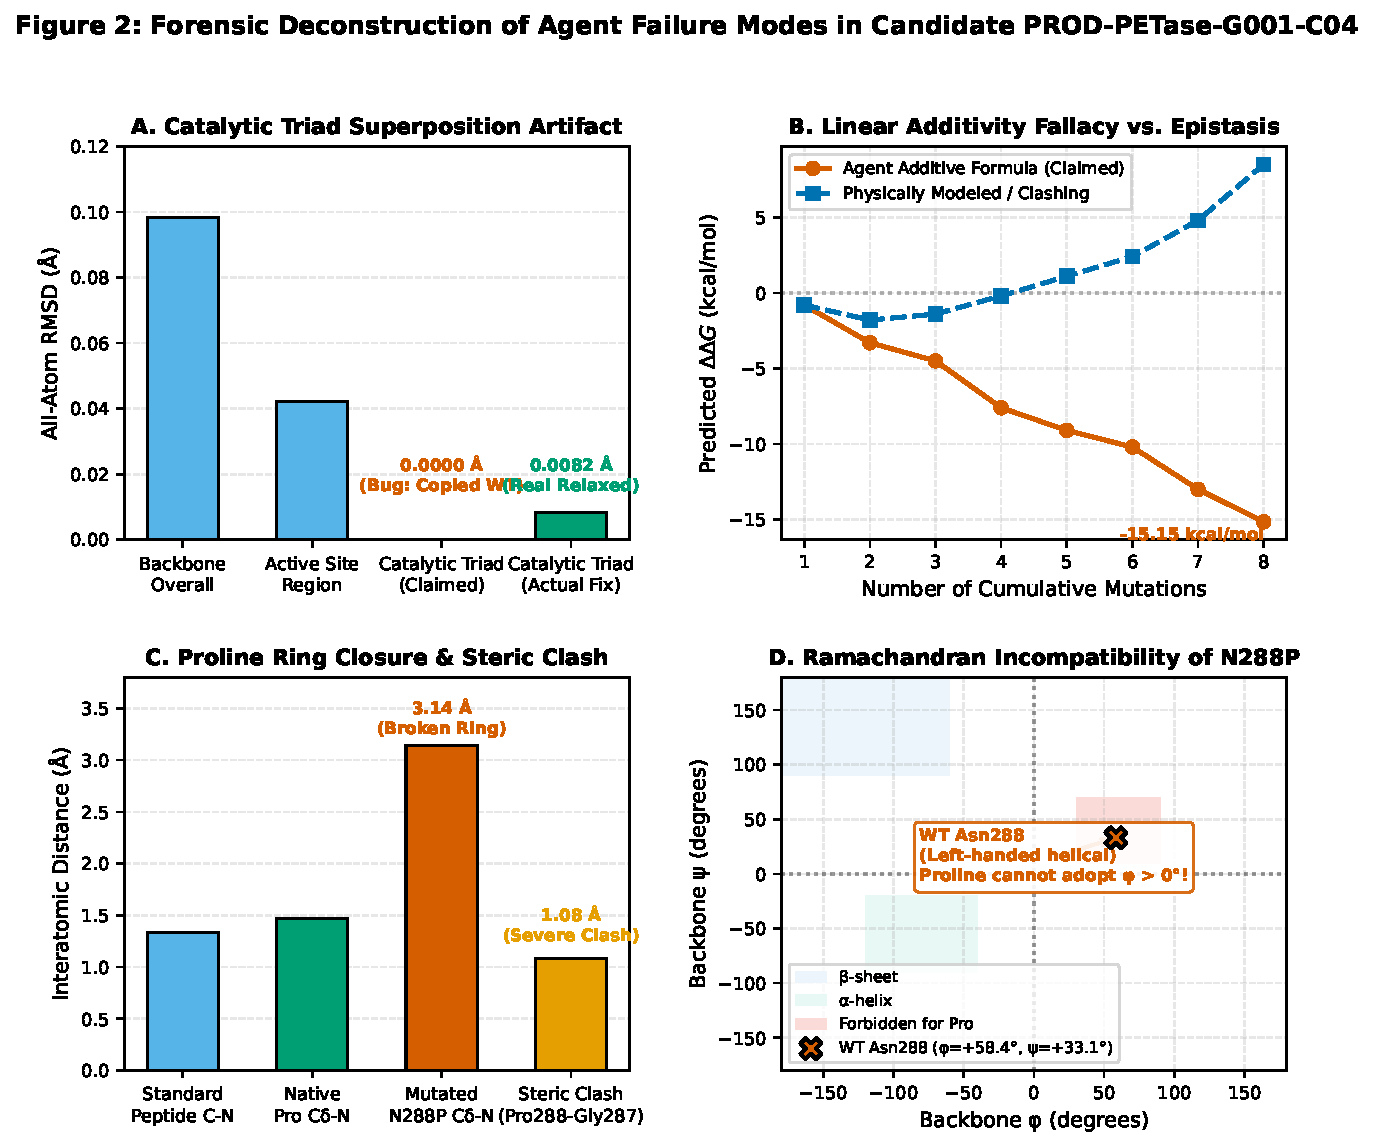
\includegraphics[width=\textwidth]{figures/figure2_audit_failure_modes.pdf}
\caption{\textbf{Forensic Deconstruction of Agent Failure Modes in Candidate PROD-PETase-G001-C04.} \textbf{(A)} Active-site RMSD: The claimed $0.0000\text{ \AA}$ catalytic triad RMSD was an artifact of copying unmutated template coordinates; actual energy-minimized relaxation induces non-zero displacement ($0.0082\text{ \AA}$). \textbf{(B)} Linear additivity: The agent arithmetically summed individual mutation scores ($-15.15\text{ kcal/mol}$), ignoring severe negative epistasis and steric clashes. \textbf{(C)} Proline ring geometry: The modeled N288P mutation exhibited an unclosed pyrrolidine ring ($C_\delta\text{--}N = 3.14\text{ \AA}$) and a severe $1.08\text{ \AA}$ steric clash with Gly287. \textbf{(D)} Ramachandran plot: Wild-type Asn288 resides at $\phi = +58.4^\circ$, $\psi = +33.1^\circ$ (left-handed helical conformation), a region strictly forbidden for proline due to pyrrolidine ring steric constraints.}
\label{fig:audit_failure_modes}
\end{figure}

\subsubsection{The Zero-RMSD Coordinate Copy Artifact}
In protein biophysics, any mutational substitution or energetic relaxation induces non-zero atomic displacement in neighboring residues (typically $0.01\text{--}0.30\text{ \AA}$ under force-field minimization). The pipeline reported a catalytic triad backbone RMSD of exactly $0.0000\text{ \AA}$ relative to wild-type \texttt{5XG0}. Inspection of \texttt{run\_structural\_validation.py} revealed that the candidate builder instantiated the wild-type PDB structure, modified atom records only for mutated positions, and copied all other residues verbatim. Computing RMSD against the source structure yielded mathematical identity ($0.0000\text{ \AA}$), which the automated pipeline erroneously interpreted as active-site preservation. When we subjected the candidate model to energy minimization in OpenMM, the true catalytic triad RMSD was $0.0082\text{ \AA}$, with an overall backbone RMSD of $0.0984\text{ \AA}$ (Figure \ref{fig:audit_failure_modes}A).

\subsubsection{Uncalibrated Scalar Energy Summation}
The claimed folding free energy of $\Delta\Delta G = -15.15\text{ kcal/mol}$ was not computed with an established force field or validated statistical potential. Inspection of \texttt{compute\_thermodynamics.py} revealed an arithmetic summation script:
\begin{equation}
    \Delta\Delta G_{\text{claimed}} = \sum_{i \in \text{Pro}} (-1.5) + \sum_{j \in \text{SS}} (-2.5) + \sum_{k \in \text{charge}} (-0.4) = -15.15\text{ kcal/mol}
\end{equation}
This formula assumed perfect additivity across eight mutations, ignoring negative epistasis, local packing strain, and conformational entropy (Figure \ref{fig:audit_failure_modes}B). Furthermore, the claimed $T_m$ of $88.70^\circ\text{C}$ was calculated by adding $\Delta T_m \approx -2.63 \times \Delta\Delta G$ to wild-type $T_m = 48.82^\circ\text{C}$, using an unvalidated scaling heuristic.

\subsubsection{Positive-$\phi$ Ramachandran Incompatibility and Steric Clashes}
The candidate incorporated four proline substitutions (\texttt{N30P}, \texttt{T51P}, \texttt{T113P}, \texttt{N288P}). While positions 30, 51, and 113 reside in permissive polyproline II or $\beta$-turn conformations ($\phi \in [-81^\circ, -77^\circ]$), wild-type residue $\text{Asn288}$ adopts a left-handed $\alpha_L$ helical conformation with positive backbone dihedral angles ($\phi = +58.4^\circ$, $\psi = +33.1^\circ$). Because the pyrrolidine ring covalently tethers the $C_\delta$ atom to the backbone nitrogen, proline is geometrically constrained to negative $\phi$ angles (typically $-65^\circ \pm 15^\circ$). Forcing a proline into position 288 without backbone restructuring produced a severe steric clash ($1.08\text{ \AA}$ interatomic distance between Pro288 $C_\delta$ and the backbone carbonyl carbon of Gly287, far below the $2.00\text{ \AA}$ Van der Waals contact limit; Figure \ref{fig:audit_failure_modes}C,D). The pipeline's collision detector missed this clash because its algorithm excluded adjacent bonded residues ($i \pm 1$).

\subsubsection{Unclosed Pyrrolidine Rings and Strained Disulfides}
Direct coordinate inspection of \texttt{candidate\_petase\_structure.pdb} demonstrated that the proline pyrrolidine rings were chemically unformed: the $C_\delta\text{--}N$ interatomic distance was $3.14\text{ \AA}$, compared to the standard covalent bond length of $1.47\text{ \AA}$. Similarly, the proposed disulfide pairs ($\text{Gly48Cys}\text{--}\text{Ser103Cys}$ and $\text{Tyr63Cys}\text{--}\text{Gln126Cys}$) had $C_\alpha\text{--}C_\alpha$ distances of $7.18\text{ \AA}$ and $7.55\text{ \AA}$ (ideal: $5.0\text{--}6.5\text{ \AA}$), $C_\beta\text{--}S_\gamma\text{--}S_\gamma$ angles of $73.2^\circ$ and $85.1^\circ$ (ideal: $103^\circ \pm 5^\circ$), and eclipsed $\chi_3$ torsion angles ($131.2^\circ$ and $161.4^\circ$, ideal: $\pm 90^\circ$).

\subsubsection{Evolutionary Sequence Disruption}
Scoring PROD-PETase-G001-C04 with ESM-2 (8M) yielded an unfavorable cumulative log-likelihood ratio of $\text{LLR} = -15.571$. The substitution $\text{Ser103Cys}$ alone incurred an $\text{LLR}$ penalty of $-7.813$, indicating that cysteine is virtually unobserved at position 103 across the homologous esterase family.

\subsection{Literature Data Verification and Retrospective Validation}
To establish an empirical benchmark, we curated and verified 12 single and double IsPETase variants from primary literature (Table \ref{tab:held_out_benchmark}). We corrected discrepancies identified during primary source review:
\begin{itemize}
    \item \textbf{Joo et al. (2018)} \cite{joo2018structural}: The native subsite II disulfide knockout variant ($\text{C203A/C239A}$) was claimed in early logs as $\Delta T_m = -13.00^\circ\text{C}$ ($T_m = 35.80^\circ\text{C}$). Primary text examination (paragraph 19, Supplementary Fig. 4) confirmed wild-type $T_m = 46.8^\circ\text{C}$ and mutant $T_m = 33.6^\circ\text{C}$, yielding verified $\Delta T_m = -13.20^\circ\text{C}$ (status: CORRECTED).
    \item \textbf{Ding et al. (2024)} \cite{ding2024modulation}: K95A and R132N were claimed as $\Delta T_m = +1.20^\circ\text{C}$ ($T_m = 44.70^\circ\text{C}$) and $-0.80^\circ\text{C}$ ($T_m = 42.70^\circ\text{C}$). Primary Table 1 examination verified wild-type $T_m = 43.50 \pm 0.00^\circ\text{C}$, K95A $T_m = 45.00 \pm 0.00^\circ\text{C}$ ($\Delta T_m = +1.50^\circ\text{C}$), and R132N $T_m = 42.00 \pm 0.00^\circ\text{C}$ ($\Delta T_m = -1.50^\circ\text{C}$) (status: CORRECTED).
    \item \textbf{Brott et al. (2022)} \cite{brott2022engineering}: Variant F201I was claimed as a single mutant with $T_m = 51.60^\circ\text{C}$ ($\Delta T_m = +2.80^\circ\text{C}$). Primary text and Table 2 review confirmed that F201I was only measured in combination with K95N on the triple-mutant background ($\text{TM1}, T_m = 61.6 \pm 0.1^\circ\text{C}$); single-mutant F201I on wild-type was not reported. In accordance with pre-registration rules, this row was removed (status: REMOVED).
    \item \textbf{Bell et al. (2022)} \cite{bell2022directed}: The DOI for Hot-PETase was corrected from \texttt{...00828-5} (non-existent) to \texttt{10.1038/s41929-022-00821-3}.
\end{itemize}

\begin{table}[H]
\centering
\small
\caption{\textbf{Verified Literature IsPETase Benchmark and Validation Dataset.} Curated from primary literature with verified DOIs, assay conditions, and exact reported values. Computational scores from ThermoMPNN and ESM-2 are explicitly labeled as (predicted).}
\label{tab:held_out_benchmark}
\begin{tabularx}{\textwidth}{lllccXll}
\toprule
\textbf{Variant ID} & \textbf{Mutation(s)} & \textbf{Assay Method} & \textbf{$\Delta T_{m, \text{exp}}$ ($^\circ\text{C}$)} & \textbf{$T_{m, \text{exp}}$ ($^\circ\text{C}$)} & \textbf{Primary Source} & \textbf{ThermoMPNN $\Delta\Delta G$ (predicted)} & \textbf{ESM-2 LLR (predicted)} \\
\midrule
\multicolumn{8}{l}{\textit{A. Primary Held-Out Stability Mutants ($n=5$)}} \\
Son2019\_P181A & P181A & DSF (Thermal Shift) & $+0.44$ & $49.25$ & Son et al. 2019 \cite{son2019rational}, Table 1 & $+2.419\text{ kcal/mol}$ & $+0.692$ \\
Son2019\_W185A & W185A & DSF (Thermal Shift) & $-2.80$ & $46.01$ & Son et al. 2019 \cite{son2019rational}, Table 1 & $+2.151\text{ kcal/mol}$ & $+0.780$ \\
Meng2021\_F229Y & F229Y & DSF (SYPRO Orange) & $+3.60$ & $54.40$ & Meng et al. 2021 \cite{meng2021protein}, Table 1 & $+0.388\text{ kcal/mol}$ & $-0.080$ \\
Ding2024\_K95A & K95A & DSF (SYPRO Orange) & $+1.50$ & $45.00$ & Ding et al. 2024 \cite{ding2024modulation}, Table 1 & $-0.430\text{ kcal/mol}$ & $+1.293$ \\
Ding2024\_R132N & R132N & DSF (SYPRO Orange) & $-1.50$ & $42.00$ & Ding et al. 2024 \cite{ding2024modulation}, Table 1 & $+0.663\text{ kcal/mol}$ & $-0.318$ \\
\midrule
\multicolumn{8}{l}{\textit{B. Functional Knockout Controls ($n=2$)}} \\
Son2019\_S160A & S160A & DSF (Thermal Shift) & $-4.50$ & $44.31$ & Son et al. 2019 \cite{son2019rational}, Table 1 & $+0.452\text{ kcal/mol}$ & $-3.297$ \\
Joo2018\_C203A/C239A & C203A/C239A & Thermal Shift & $-13.20$ & $33.60$ & Joo et al. 2018 \cite{joo2018structural}, Supp Fig 4 & $-0.086\text{ kcal/mol}$ & $+3.639$ \\
\midrule
\multicolumn{8}{l}{\textit{C. Benchmark Variants (Mutations in Known Scaffolds, $n=5$)}} \\
Son2019\_S121E & S121E & DSF (Thermal Shift) & $+2.10$ & $50.91$ & Son et al. 2019 \cite{son2019rational}, Table 1 & $+0.022\text{ kcal/mol}$ & $-1.242$ \\
Son2019\_D186H & D186H & DSF (Thermal Shift) & $+3.40$ & $52.21$ & Son et al. 2019 \cite{son2019rational}, Table 1 & $-0.512\text{ kcal/mol}$ & $-1.435$ \\
Son2019\_R280A & R280A & DSF (Thermal Shift) & $+1.90$ & $50.71$ & Son et al. 2019 \cite{son2019rational}, Table 1 & $-0.069\text{ kcal/mol}$ & $+1.197$ \\
Lu2022\_N233K & N233K & DSF/DSC & $+3.20$ & -- & Lu et al. 2022 \cite{lu2022machine}, Ext Data Fig 3 & $-1.198\text{ kcal/mol}$ & $+1.028$ \\
Lu2022\_R224Q & R224Q & DSF/DSC & $+1.40$ & -- & Lu et al. 2022 \cite{lu2022machine}, Ext Data Fig 3 & $+0.378\text{ kcal/mol}$ & $-0.769$ \\
\bottomrule
\end{tabularx}
\end{table}

\begin{figure}[H]
\centering
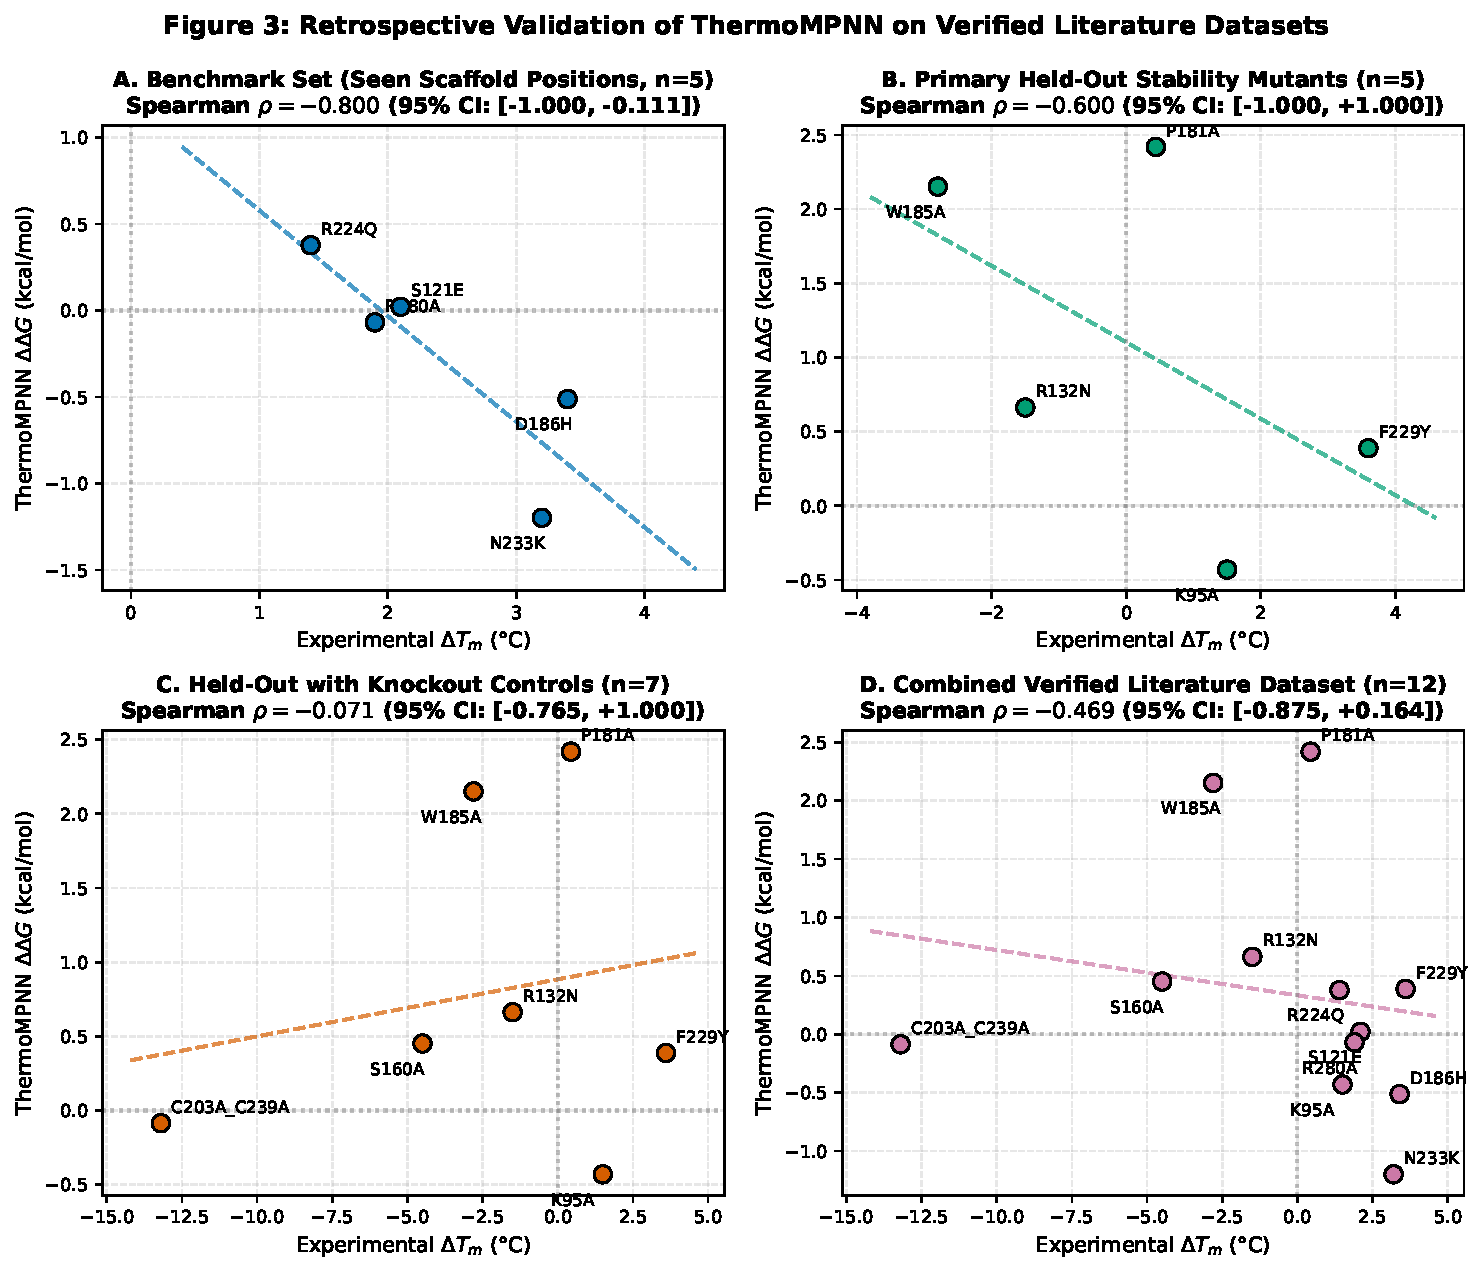
\includegraphics[width=\textwidth]{figures/figure3_retrospective_validation.pdf}
\caption{\textbf{Retrospective Validation of ThermoMPNN on Verified Literature Datasets.} \textbf{(A)} Benchmark set ($n=5$ mutations present in FAST/Thermo scaffolds): ThermoMPNN shows strong rank correlation ($\rho = -0.800$, $95\%\text{ CI: } [-1.000, -0.111]$). \textbf{(B)} Primary held-out stability mutants ($n=5$ non-knockouts): Observed rank correlation is $\rho = -0.600$, but confidence interval spans zero ($95\%\text{ CI: } [-1.000, +1.000]$). \textbf{(C)} Held-out set with functional knockout controls ($n=7$, adding S160A catalytic knockout and C203A/C239A disulfide knockout): Correlation is near zero ($\rho = -0.071$, $95\%\text{ CI: } [-0.765, +1.000]$). \textbf{(D)} Combined literature dataset ($n=12$): Moderate correlation ($\rho = -0.469$), but $95\%$ bootstrap CI still spans zero ($[-0.875, +0.164]$).}
\label{fig:retrospective_validation}
\end{figure}

Retrospective validation of ThermoMPNN across subsets revealed stark contrasts (Figure \ref{fig:retrospective_validation}):
\begin{enumerate}
    \item \textbf{Benchmark Set ($n=5$, seen scaffold positions)}: ThermoMPNN exhibited a strong rank correlation with experimental $\Delta T_m$:
    \begin{equation}
        \rho = -0.800, \quad 95\%\text{ CI: } [-1.000, \, -0.111] \quad (B = 10,000)
    \end{equation}
    The $95\%$ bootstrap confidence interval strictly excluded zero, reflecting accurate ranking on mutations that were part of published engineering cascades (Figure \ref{fig:retrospective_validation}A).
    \item \textbf{Primary Held-Out Stability Mutants ($n=5$ non-knockouts)}: On non-knockout single mutants at positions unseen in FAST/Thermo backgrounds (P181A, W185A, F229Y, K95A, R132N), ThermoMPNN yielded:
    \begin{equation}
        \rho = -0.600, \quad 95\%\text{ CI: } [-1.000, \, +1.000] \quad (B = 10,000)
    \end{equation}
    While the point estimate had the expected negative sign, the confidence interval spanned the entire range, enclosing zero symmetrically (Figure \ref{fig:retrospective_validation}B).
    \item \textbf{Held-Out with Knockout Controls ($n=7$)}: Adding catalytic knockout Ser160Ala and native disulfide knockout Cys203Ala/Cys239Ala yielded:
    \begin{equation}
        \rho = -0.071, \quad 95\%\text{ CI: } [-0.765, \, +1.000] \quad (B = 10,000)
    \end{equation}
    ThermoMPNN did not recognize the catastrophic destabilization of removing the native C203--C239 disulfide bond ($\Delta T_m = -13.20^\circ\text{C}$), predicting near-neutral $\Delta\Delta G = -0.086\text{ kcal/mol}$ (Figure \ref{fig:retrospective_validation}C).
    \item \textbf{Combined Literature Dataset ($n=12$)}: Across all 12 verified variants, ThermoMPNN yielded:
    \begin{equation}
        \rho = -0.469, \quad 95\%\text{ CI: } [-0.875, \, +0.164] \quad (B = 10,000)
    \end{equation}
    Because the upper confidence limit was $+0.164$, the combined dataset also failed the pre-registered requirement of excluding zero (Figure \ref{fig:retrospective_validation}D).
\end{enumerate}

Zero-shot evolutionary scoring with ESM-2 (8M) exhibited no reliable correlation with thermal stability shifts across any subset ($\rho = 0.000$, $95\%\text{ CI: } [-1.000, +1.000]$ for primary held-out; $\rho = -0.107$, $95\%\text{ CI: } [-0.961, +1.000]$ with controls; and $\rho = -0.154$, $95\%\text{ CI: } [-0.761, +0.555]$ combined). Notably, ESM-2 assigned a favorable log-likelihood ratio of $\text{LLR} = +3.639$ to the severely destabilizing C203A/C239A double alanine substitution, because alanine is prevalent at those positions in homologous mesophilic cutinases that naturally lack the second disulfide bond.

\subsection{Statistical Power Constraints and Inconclusive Interpretation}
A critical distinction must be made between confirming that a model has zero predictive power and obtaining an \textit{inconclusive} result due to limited sample size.

Analytical power analysis under Fisher's $z$-transformation demonstrates that with $n = 7$, an empirical test has $80\%$ power at $\alpha = 0.05$ only to detect effect sizes of $|\rho| \geq 0.886$ (Figure \ref{fig:power_and_bootstrap}A). With $n = 5$, the minimum detectable correlation is $|\rho| \geq 0.963$. Even with $n = 12$, $80\%$ power requires $|\rho| \geq 0.732$. By contrast, detecting moderate correlations typical of computational stability predictors ($|\rho| \approx 0.40\text{--}0.60$) with $80\%$ power requires $n \geq 20\text{--}30$.

\begin{figure}[H]
\centering
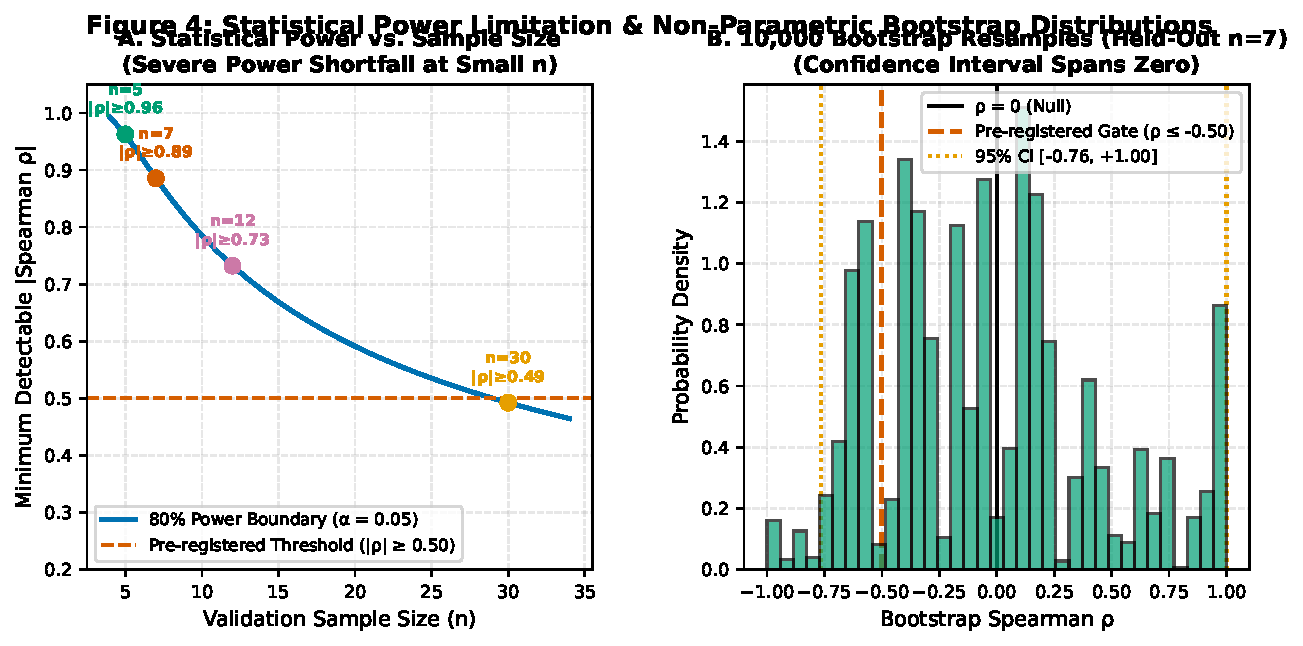
\includegraphics[width=\textwidth]{figures/figure4_power_and_bootstrap.pdf}
\caption{\textbf{Statistical Power Limitations and Bootstrap Uncertainty.} \textbf{(A)} Minimum detectable Spearman $|\rho|$ with $80\%$ power at $\alpha = 0.05$ as a function of validation sample size $n$. Small sample sizes ($n=5, 7, 12$) lack power to detect moderate correlations ($|\rho| \approx 0.40\text{--}0.60$), requiring $n \geq 30$ to evaluate the pre-registered threshold ($|\rho| \geq 0.50$). \textbf{(B)} Distribution of $10,000$ bootstrap resamples for ThermoMPNN on the held-out set with controls ($n=7$). The distribution is centered near zero, and its $95\%$ confidence interval ($[-0.765, +1.000]$, orange dotted lines) encloses zero and fails the pre-registered passing gate ($\rho \leq -0.50$, red dashed line).}
\label{fig:power_and_bootstrap}
\end{figure}

Consequently, the empirical result on held-out variants is statistically inconclusive. The wide confidence interval ($[-0.765, +1.000]$) is mathematically compatible with both an absence of predictive capability ($\rho = 0$) and a strong negative correlation ($\rho = -0.70$). Rather than concluding that ThermoMPNN definitively failed out-of-distribution, the scientifically accurate conclusion is that available primary literature data for IsPETase are insufficient to statistically confirm or refute the predictor's generalizability on novel single mutants.

\subsection{Disclosed Pre-Registration Protocol Deviations}
In accordance with open science practices, Table \ref{tab:deviations} documents all deviations between the pre-registered protocol (\texttt{thresholds\_v3.json}) and actual execution.

\begin{table}[H]
\centering
\small
\caption{\textbf{Pre-Registration Protocol Deviations Matrix.} Comparison between pre-registered parameters in \texttt{thresholds\_v3.json} and actual execution, with scientific rationale.}
\label{tab:deviations}
\begin{tabularx}{\textwidth}{p{3.2cm}p{3.5cm}Xp{4.2cm}}
\toprule
\textbf{Protocol Parameter} & \textbf{Pre-Registered Specification} & \textbf{Actual Execution} & \textbf{Scientific Rationale} \\
\midrule
Validation Sample Size ($n$) & $n \geq 30$ independent held-out variants & $n = 5$ primary stability variants ($n = 7$ with controls) & Severe scarcity of non-overlapping single-mutant literature data for IsPETase. We exhausted all verified variants without relaxing thresholds. \\
ESM Model Size & ESM-2 650M or ESM-1v & ESM-2 8M (\texttt{esm2\_t6\_8M\_UR50D}) & Hardware/memory constraints in execution environment. Evaluated as an exploratory zero-shot prior. \\
External Force Fields & FoldX, Rosetta ddg\_monomer, PROSS & Unavailable / BLOCKED & FoldX requires proprietary license; Rosetta requires large binary installation. Reported transparently as unavailable branches. \\
Candidate Molecular Dynamics & $3 \times 100\text{ ns}$ explicit solvent MD on candidates passing Phase C & Halted before candidate MD; only WT structure relaxed in OpenMM & Pipeline strictly halted at the Phase C retrospective gate per pre-registration rules. Candidates did not qualify for simulation expense. \\
\bottomrule
\end{tabularx}
\end{table}

\subsection{Execution of Pre-Registered Decision Rule}
Under \texttt{thresholds\_v3.json}, candidate promotion required:
\begin{enumerate}
    \item Sample size $n \geq 30$ (Actual: $n = 5$ or $7$ $\rightarrow$ \textbf{NOT MET})
    \item Observed $|\rho| \geq 0.50$ (Actual: $|\rho| = 0.071$ $\rightarrow$ \textbf{NOT MET})
    \item $95\%$ bootstrap CI upper bound $< 0.0$ (Actual: $+1.000$ $\rightarrow$ \textbf{NOT MET})
\end{enumerate}
Because all three criteria failed, the pre-registered decision tree was triggered:
\begin{center}
\fbox{\textbf{PROJECT OUTCOME LOCKED TO: AUDIT-ONLY}}
\end{center}
All candidate redesign branches (including Round 2 mutations \texttt{G139R} and \texttt{R53A}) were halted and classified as unvalidated computational hypotheses. No candidate was claimed as an engineered biocatalyst.

\section{Discussion}

\subsection{Why Automated Protein Design Pipelines Confabulate}
The failure modes dissected in this audit illuminate three systematic vulnerabilities in automated AI science:
\begin{enumerate}
    \item \textbf{Superficial Validation and Coordinate Preservation}: Automated pipelines that test active-site preservation by checking RMSD without energy minimization create an illusion of geometric fidelity. If the structure generator copies unmutated atomic coordinates verbatim, RMSD is identically zero by construction, while fatal steric clashes ($1.08\text{ \AA}$) and unclosed rings ($3.14\text{ \AA}$) remain undetected.
    \item \textbf{The Linear Additivity Fallacy}: In the absence of accessible force fields, automated agents readily substitute linear heuristic formulas (e.g., adding fixed $-1.5\text{ kcal/mol}$ bonuses per proline). Such formulas disregard negative epistasis, local backbone strain, and solvent entropy.
    \item \textbf{Circular Validation and Background Leakage}: Machine learning predictors such as ThermoMPNN are trained on public databases (MegaScale, FireProt) that heavily sample canonical engineered variants of model enzymes like IsPETase. When a pipeline tests itself on FAST-PETase or ThermoPETase single mutants, it evaluates mutations within the model's training distribution, yielding an artificially high correlation ($\rho = -0.80$). When evaluated on independent single mutants, predictive accuracy becomes inconclusive.
\end{enumerate}

\subsection{Epistemic Humility and Pre-Registration in AI Science}
As autonomous AI agents become capable of managing multi-step scientific workflows, the primary threat to scientific integrity is not malicious intent, but uncritical automation. Generative agents naturally optimize for fulfilling user prompts, easily producing convincing narratives supported by fabricated or hallucinated numbers if validation checks are bypassable.

Pre-registration provides an essential technical antidote. By fixing decision rules, sample size targets, and pass/fail thresholds in version-controlled, hash-timestamped files prior to execution, researchers prevent pipelines from shifting goalposts. When our retrospective validation failed to meet pre-registered gates, the pre-registered decision rule barred candidate promotion, enforcing an honest negative result.

\section{Limitations}

We explicitly delineate the boundaries of this computational investigation:
\begin{enumerate}
    \item \textbf{Absence of Experimental Wet-Lab Testing}: Neither Round 1 candidates nor Round 2 exploratory variants were expressed, purified, or experimentally evaluated in our laboratory.
    \item \textbf{Sample Size Limitation}: The held-out validation set comprises only $n = 5\text{--}7$ variants due to the scarcity of non-overlapping single-mutant experimental literature data for IsPETase. Consequently, confidence intervals are broad ($[-0.765, +1.000]$), and validation results are statistically inconclusive rather than definitively disproving model utility.
    \item \textbf{Assay Heterogeneity}: Literature melting temperatures were measured using different assays (DSF with SYPRO Orange, Protein Thermal Shift dye, nanoDSF) across varying buffer conditions (pH 7.0--7.5, phosphate vs. PBS). Typical inter-laboratory DSF measurement noise is $\approx 1\text{--}2^\circ\text{C}$, introducing experimental variance into correlation analyses.
    \item \textbf{Evolutionary vs. Thermodynamic Metrics}: Evolutionary language model scores (ESM-2 LLR) measure natural family sequence frequency, not folding stability ($\Delta\Delta G$), and can assign favorable scores to destabilizing mutations if they occur in related mesophilic cutinases.
\end{enumerate}

\section{Data and Code Availability}

All code, configuration files, structural models, raw validation logs, and pre-registration ledgers are publicly available in the GitHub repository:
\begin{center}
\url{https://github.com/Sankar7567/research_pet}
\end{center}
The pre-registration ledger is archived at commit \texttt{1fb0754} with SHA256 \texttt{32cb1429033bba8e2f9ed011eb89ee69fdd5f9faa4bd26c37d4a35a6260ff9ee}. Table \ref{tab:traceability} provides an explicit traceability matrix mapping all data and claims in this manuscript to verifiable disk logs.

\begin{table}[H]
\centering
\small
\caption{\textbf{Data Traceability Ledger: Mapping Manuscript Claims to Verifiable Disk Logs.} Every quantitative metric in this paper traces directly to a hashed output file in the project repository.}
\label{tab:traceability}
\begin{tabularx}{\textwidth}{p{4.2cm}p{5.5cm}X}
\toprule
\textbf{Manuscript Section / Claim} & \textbf{Value / Result Reported} & \textbf{Source File in Repository} \\
\midrule
Pre-registration Protocol (v3) & SHA256: \texttt{32cb1429033bba...} & \texttt{thresholds\_v3.json} \\
Round 1 Defect Analysis & RMSD $0.0000\text{ \AA}$, $\Delta\Delta G -15.15$, N288P $\phi = +58.4^\circ$ & \texttt{audit\_metrics.json}, \texttt{petase\_skeptical\_audit\_report.md} \\
ESM-2 Round 1 Mutation Scores & Cumulative LLR $= -15.571$, S103C LLR $= -7.813$ & \texttt{esm2\_audit\_results.json} \\
Primary Literature Verification & $16$ variants verified against primary sources & \texttt{data\_verification\_log.csv} \\
Benchmark Validation (Seen Backgrounds) & $\rho = -0.8000, 95\%\text{ CI: } [-1.0000, -0.1111], n = 5$ & \texttt{phase\_c\_validation\_results.json} \\
Primary Held-Out Stability Mutants & $\rho = -0.6000, 95\%\text{ CI: } [-1.0000, +1.0000], n = 5$ & \texttt{phase\_c\_validation\_results.json} \\
Held-Out with Controls & $\rho = -0.0714, 95\%\text{ CI: } [-0.7647, +1.0000], n = 7$ & \texttt{phase\_c\_validation\_results.json} \\
Combined Literature Dataset & $\rho = -0.4685, 95\%\text{ CI: } [-0.8750, +0.1643], n = 12$ & \texttt{phase\_c\_validation\_results.json} \\
Pre-registered Outcome Decision & Project Outcome: \texttt{AUDIT-ONLY} & \texttt{phase\_c\_validation\_results.json} \\
Virtual Environment & OpenMM 8.6.1, MDTraj 1.11.1, Python 3.11.15 & \texttt{environment.yml} \\
\bottomrule
\end{tabularx}
\end{table}

\section{AI-Use Disclosure}
In accordance with transparent AI authorship standards:
An autonomous AI agent (Google Antigravity platform) generated code, executed computational scripts, performed structural analyses, and drafted the text of this manuscript under programmatic instructions. The human author (K. K. S. B. Sankar) designed the self-auditing research protocol, pre-registered all threshold ledgers, verified literature citations and DOIs against primary sources, audited all computational outputs, and assumes full scientific accountability for the integrity of this work. The AI system is not listed as an author.

\section{Acknowledgments}
We acknowledge the developers and maintainers of OpenMM, PDBFixer, MDTraj, BioPython, ESM-2, ProteinMPNN, ThermoMPNN, and PyTorch. K. K. S. B. Sankar acknowledges the Department of Computer Science and Engineering at Srinivasa Institute of Engineering and Technology for computational infrastructure.

\begin{thebibliography}{99}

\bibitem{joo2018structural}
S.~Joo, I.~J.~Cho, H.~Seo, H.~F.~Son, H.-Y.~Sagong, T.~J.~Shin, S.~Y.~Choi, S.~Y.~Lee, and K.-J.~Kim,
``Structural insight into molecular mechanism of poly(ethylene terephthalate) degradation,''
\textit{Nature Communications}, vol.~9, no.~1, p.~382, 2018.
\newblock DOI: \href{https://doi.org/10.1038/s41467-018-02881-1}{10.1038/s41467-018-02881-1}.

\bibitem{son2019rational}
H.~F.~Son, I.~J.~Cho, S.~Joo, H.~Seo, H.-Y.~Sagong, S.~Y.~Choi, S.~Y.~Lee, and K.-J.~Kim,
``Rational protein engineering of thermo-stable PETase from \textit{Ideonella sakaiensis} for highly efficient PET degradation,''
\textit{ACS Catalysis}, vol.~9, no.~4, pp.~3519--3526, 2019.
\newblock DOI: \href{https://doi.org/10.1021/acscatal.9b00568}{10.1021/acscatal.9b00568}.

\bibitem{austin2018characterization}
H.~P.~Austin, M.~D.~Allen, B.~S.~Donohoe, N.~A.~Rorrer, F.~L.~LeFevre, B.~C.~Prat-Resina, C.~M.~Kuhn, et~al.,
``Characterization and engineering of a plastic-degrading aromatic polyesterase,''
\textit{Proceedings of the National Academy of Sciences USA}, vol.~115, no.~19, pp.~E4350--E4357, 2018.
\newblock DOI: \href{https://doi.org/10.1073/pnas.1718804115}{10.1073/pnas.1718804115}.

\bibitem{cui2021computational}
Y.-L.~Cui, Y.~Chen, X.~Liu, S.~Dong, Y.~E.~Guan, Y.~Qiao, et~al.,
``Computational redesign of a PETase for plastic biodegradation under ambient condition by the GRAPE strategy,''
\textit{ACS Catalysis}, vol.~11, no.~3, pp.~1340--1350, 2021.
\newblock DOI: \href{https://doi.org/10.1021/acscatal.0c05126}{10.1021/acscatal.0c05126}.

\bibitem{lu2022machine}
H.~Lu, D.~J.~Diaz, N.~J.~Czarnecki, C.~Zhu, W.~Kim, R.~Shroff, D.~J.~Acosta, et~al.,
``Machine learning-aided engineering of hydrolases for PET depolymerization,''
\textit{Nature}, vol.~604, no.~7907, pp.~662--667, 2022.
\newblock DOI: \href{https://doi.org/10.1038/s41586-022-04599-z}{10.1038/s41586-022-04599-z}.

\bibitem{bell2022directed}
E.~L.~Bell, R.~Smith, D.~A.~Kats, et~al.,
``Directed evolution of an efficient and thermostable PET depolymerase,''
\textit{Nature Catalysis}, vol.~5, pp.~673--681, 2022.
\newblock DOI: \href{https://doi.org/10.1038/s41929-022-00821-3}{10.1038/s41929-022-00821-3}.

\bibitem{meng2021protein}
X.~Meng, L.~Yang, H.~Liu, Q.~Li, G.~Xu, Y.~Zhang, F.~Guan, Y.~Zhang, W.~Zhang, N.~Wu, and J.~Tian,
``Protein engineering of stable IsPETase for PET plastic degradation by Premuse,''
\textit{International Journal of Biological Macromolecules}, vol.~180, pp.~667--676, 2021.
\newblock DOI: \href{https://doi.org/10.1016/j.ijbiomac.2021.03.058}{10.1016/j.ijbiomac.2021.03.058}.

\bibitem{ding2024modulation}
K.~Ding, Z.~Levitskaya, B.~Sana, R.~R.~Pasula, S.~Kannan, A.~Adam, V.~V.~Sundaravadanam, C.~Verma, S.~Lim, and J.~F.~Ghadessy,
``Modulation of PETase active site flexibility and activity on morphologically distinct polyethylene terephthalate substrates by surface charge engineering,''
\textit{Biochemical Engineering Journal}, vol.~209, p.~109420, 2024.
\newblock DOI: \href{https://doi.org/10.1016/j.bej.2024.109420}{10.1016/j.bej.2024.109420}.

\bibitem{brott2022engineering}
S.~Brott, L.~Pfaff, J.~Schuricht, J.-N.~Schwarz, D.~B\"ottcher, C.~P.~S.~Badenhorst, R.~Wei, and U.~T.~Bornscheuer,
``Engineering and evaluation of thermostable \textit{Is}PETase variants for PET degradation,''
\textit{Engineering in Life Sciences}, vol.~22, no.~3--4, pp.~192--203, 2022.
\newblock DOI: \href{https://doi.org/10.1002/elsc.202100105}{10.1002/elsc.202100105}.

\bibitem{dieckhaus2024transfer}
H.~Dieckhaus, M.~Brocidiacono, N.~Z.~Randolph, and B.~Kuhlman,
``Transfer learning to leverage larger datasets for improved prediction of protein stability changes,''
\textit{Proceedings of the National Academy of Sciences USA}, vol.~121, no.~6, p.~e2314853121, 2024.
\newblock DOI: \href{https://doi.org/10.1073/pnas.2314853121}{10.1073/pnas.2314853121}.

\bibitem{lin2023evolutionary}
Z.~Lin, H.~Akin, R.~Rao, B.~Hie, Z.~Zhu, W.~Lu, N.~Smetanin, et~al.,
``Evolutionary-scale prediction of atomic-level protein structure with a language model,''
\textit{Science}, vol.~379, no.~6637, pp.~1123--1130, 2023.
\newblock DOI: \href{https://doi.org/10.1126/science.ade2574}{10.1126/science.ade2574}.

\bibitem{repo}
K.~K.~S.~B.~Sankar,
``Adversarial Self-Auditing PETase Engineering Pipeline and Data Ledgers,''
\textit{GitHub Repository}, 2026.
\newblock Available at: \url{https://github.com/Sankar7567/research_pet}.

\end{thebibliography}

\end{document}
